\vspace{-2mm}
\section{Evaluation}


\begin{figure*}[t!]
    \centering
    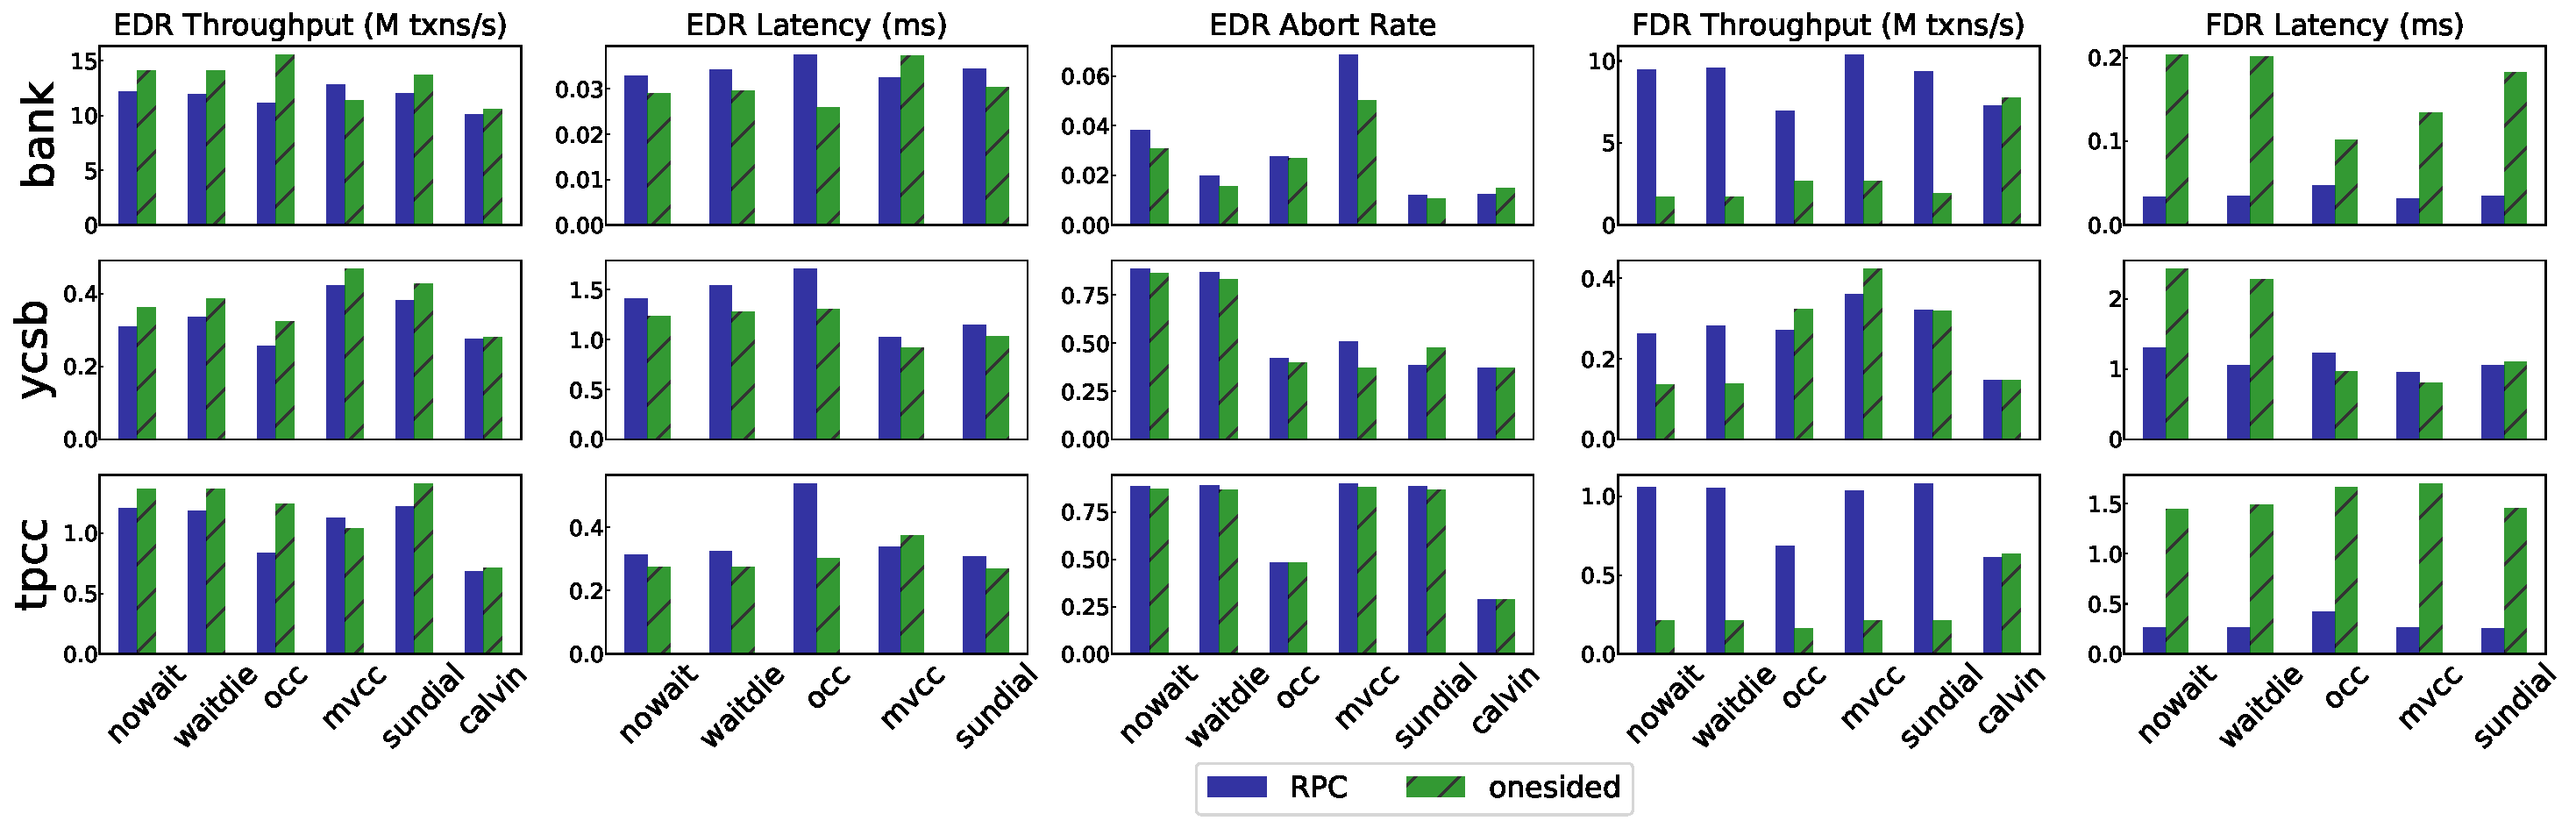
\includegraphics[width=18cm]{images/eval_overall.pdf}
    \vspace{-0.4cm}
    \caption{Overall throughput, latency for both EDR and FDR clusters and abort rates for the EDR cluster for all six protocols}
    \vspace{-0.7cm}
    \label{fig:eval_overall}
\end{figure*}

%\vspace{-2mm}
\subsection{Workloads}
%\vspace{-2mm}

We use three popular OLTP benchmarks, SmallBank~\cite{SmallBank}, YCSB~\cite{cooper2010benchmarking}, and TPC-C~\cite{TPC-C}, to test the performance of each protocol using two-sided RPC (denoted as \textbf{rpc}) or one-sided primitives (denoted as \textbf{onesided}). Records are partitioned across nodes. %To avoid effecting the results due to the assumption of locality, 
To eliminate the effects of locality, 
all transactions 
use network operations to fetch and update the data. 

\textbf{SmallBank}~\cite{SmallBank} is a simple banking application. Each transaction performs simple reads and writes on the account data. The key feature of SmallBank is that it has a small number of writes and reads in one transaction (in total less than four) with 
simple arithmetic operations.
%And its execution stage is quite simple. which is usually just one arithmetic operation. 
This makes SmallBank a network-intensive application. %Moreover, each record in SmallBank is of 4 bytes: it just stores simple information like checking and saving. It has six types of transactions, each sharing the same possibility of execution in our evaluations.

\textbf{YCSB}~\cite{cooper2010benchmarking} (The Yahoo! Cloud Serving Benchmark) is designed to evaluate large-scale Internet applications. There is just one table in the database. YCSB parameters such as
record size, the number of writes or reads involved in a transaction, the ratio of read/write and the skews are all configurable. In all our experiments, the record length is set to 64 bytes, with 1200000 entries in the table. We used hot area in YCSB, which consists of 1200 entries, i.e., 0.1\% of total records, to control contention. The number of table entries and hot area we use are proportional to the number of threads in \projectname. There are 10 operations in one transaction, with different read/write ratios.% in different experiments.
% In our test, an execution phase consuming 25\% of the whole transaction time is added to simulate the actual computation of a transaction.

\textbf{TPC-C}~\cite{TPC-C} simulates the processing of warehouse orders. In our evaluation, we run the transaction ``New-Order'', which consists of longer (up to 15) write sets and more complex transaction executions. In this benchmark, TPC-C has higher 
CPU utilization than SmallBank.

\vspace{-2mm}
\subsection{Execution Setup}
\vspace{-2mm}

We test our framework on two clusters, the first is an RDMA-capable cluster with 8 nodes. Each node is equipped with two 12-core Intel Xeon E5-2670 v3 processor, 128GB RAM and one ConnectX-4 EDR 100Gb/s InfiniBand MT27700. The second cluster is an RDMA-capable cluster with 16 nodes. Each node has two 8-core Intel Xeon CPU E5-2630 v3 processors, 64GB RAM, and one ConnectX-3 Pro FDR 56Gb/s InfiniBand MT27520. As there is only one RNIC on each node, we only run evaluations on the CPU on the same NUMA node with the RNIC to prevent NUMA from affecting our results. We name the first cluster EDR and the second cluster FDR in our experiments. We evaluate both \textbf{RPC} and \textbf{onesided} implementations of all \projectname protocols and focus on three metrics: {\em throughput, latency and abort rate}. To focus on comparing communication styles and protocols, we enforce coordinators to self-generate transaction requests.

\vspace{-2mm}
\subsection{Overall Results}
\vspace{-2mm}

% For six protocols, there are mainly three indicators to value the performance of the transaction protocol. They are throughput, latency and abort rate. These values are not independent, there are actually very complicated relationship between them.

Figure~\ref{fig:eval_overall} shows the overall results. In overall evaluations of YCSB, we have 20\% write and 80\% read and set the computation in the execution phase of YCSB to 5\% of the total latency of a transaction to simulate real-world applications. For evaluating throughput and abort rate, on the EDR cluster, we use 10 threads on each node and 10 co-routines for each thread, each co-routine producing and handling transaction requests independently. For the FDR cluster, we use 8 threads due to the limited number of cores in one CPU. %\blue{We use the }

%\begin{tcolorbox}
\underline{\bf Finding 1}: \textbf{Onesided} has a comparable or better throughput than \textbf{RPC} with only two exceptions for \mvcc on the EDR cluster (100Gb/s). 
%\end{tcolorbox}

\setlength{\intextsep}{2pt}%
\setlength{\columnsep}{8pt}%
\begin{wrapfigure}[5]{r}{.50\linewidth}
    \centering
    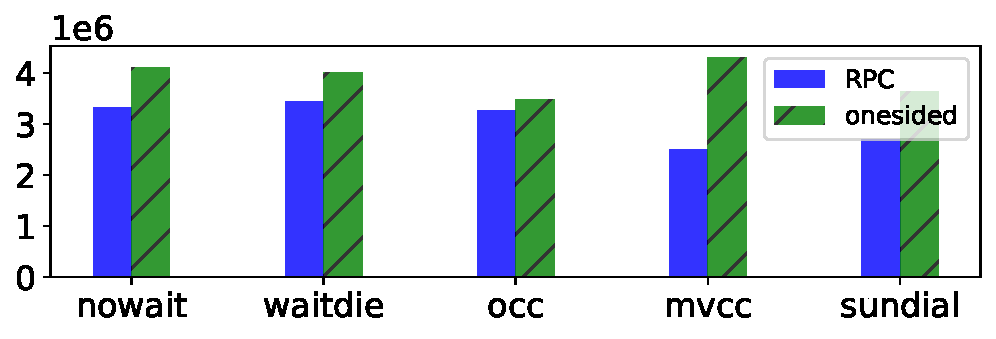
\includegraphics[width=\linewidth]{RCC-ISCA2020/images/network_trips.pdf}
    \vspace{-0.6cm}
    \caption{Network Round Trips}
    \vspace{-0.3cm}
    \label{fig:round-trips}
\end{wrapfigure}
We attribute \textit{Finding 1} to the fact that \textbf{onesided} can bypass remote CPUs, thus having a smaller communication overhead in general compared to their \textbf{RPC} counterparts for each round trip. This observation is true only when \textbf{onesided} implementations do not incur excessive amount of communication round trips compared to their \textbf{RPC} counterparts. However, this is not true for \mvcc. As we can see in Figure~\ref{fig:round-trips}, \textbf{onesided} \mvcc implementations incur 72\% more communication round trips while other protocols incur only a range of 6\% to 34\% more communication round trips. Therefore \textbf{RPC} is better than \textbf{onesided} for \mvcc on SmallBank and TPC-C. As for \mvcc on YCSB, which is a computation-intensive workload, \textbf{onesided} still dominates \textbf{RPC} even with 72\% more round trips; the advantage of bypassing remote CPUs becomes salient when remote CPUs are kept busy with computations.



%Such advantage of \textbf{onesided} becomes salient on computation-intensive workloads 
%\begin{tcolorbox}
\underline{\bf Finding 2}: While \textbf{onesided} is generally better than \textbf{RPC} on the EDR cluster (100Gb/s), \textbf{onesided} \occ is not necessarily the best protocol choice.
%\end{tcolorbox}

Protocols can be compared easily in \projectname. For SmallBank, which is a network-intensive benchmark and of low contention, \textbf{onesided} \occ is the best choice 
because it has the least number of network operations due to its optimistic assumption. For YCSB, which has more computation in the execution stage and more operations within one transaction, \textbf{onesided} \mvcc is the best. Moreover, it resolves many read-write conflicts by maintaining multiple versions of the records. So it has the lowest abort rate and highest throughput. For TPC-C, \textbf{onesided} \sundial is the best since it has the dynamic read lease and transaction timestamp. 

%\begin{tcolorbox}
\underline{\bf  Finding 3}: 
One-sided operations are not quite beneficial with 
low bandwidth (56Gb/s FDR). Only two protocols benefit from one-sided primitives under a computation-intensive workload.
%\end{tcolorbox}

%On the FDR cluster, one-sided operations are not well supported by the RNIC. 
On the FDR cluster, for read, write and lock requests, the latency of one-sided operations is 2.3x more than RPC with two-sided operations. The throughput and latency results of SmallBank shows that \textbf{RPC} is much better than \textbf{onesided} when the application is network bounded. YCSB, while having additional computation in the execution stage to increase co-routine execution time and burden remote CPUs, can still take advantage of the feature of \textbf{onesided} to bypass remote CPU and to outperform \textbf{RPC} for some protocols like \mvcc and \occ when the application is CPU-bounded. We do all experiments on the EDR cluster for later subsections.

On both clusters, the latency results essentially reflect similar conclusions as we have drawn from throughput results. As we use multiple (i.e., ten) co-routines to improve throughput, the latency of executing one transaction is adversely affected due to context switching. We will investigate latency breakdown by using just one co-routine later.

\vspace{-2mm}
\subsection{Impact of Co-routines}
\vspace{-2mm}

\begin{figure}[h]
    \centering
    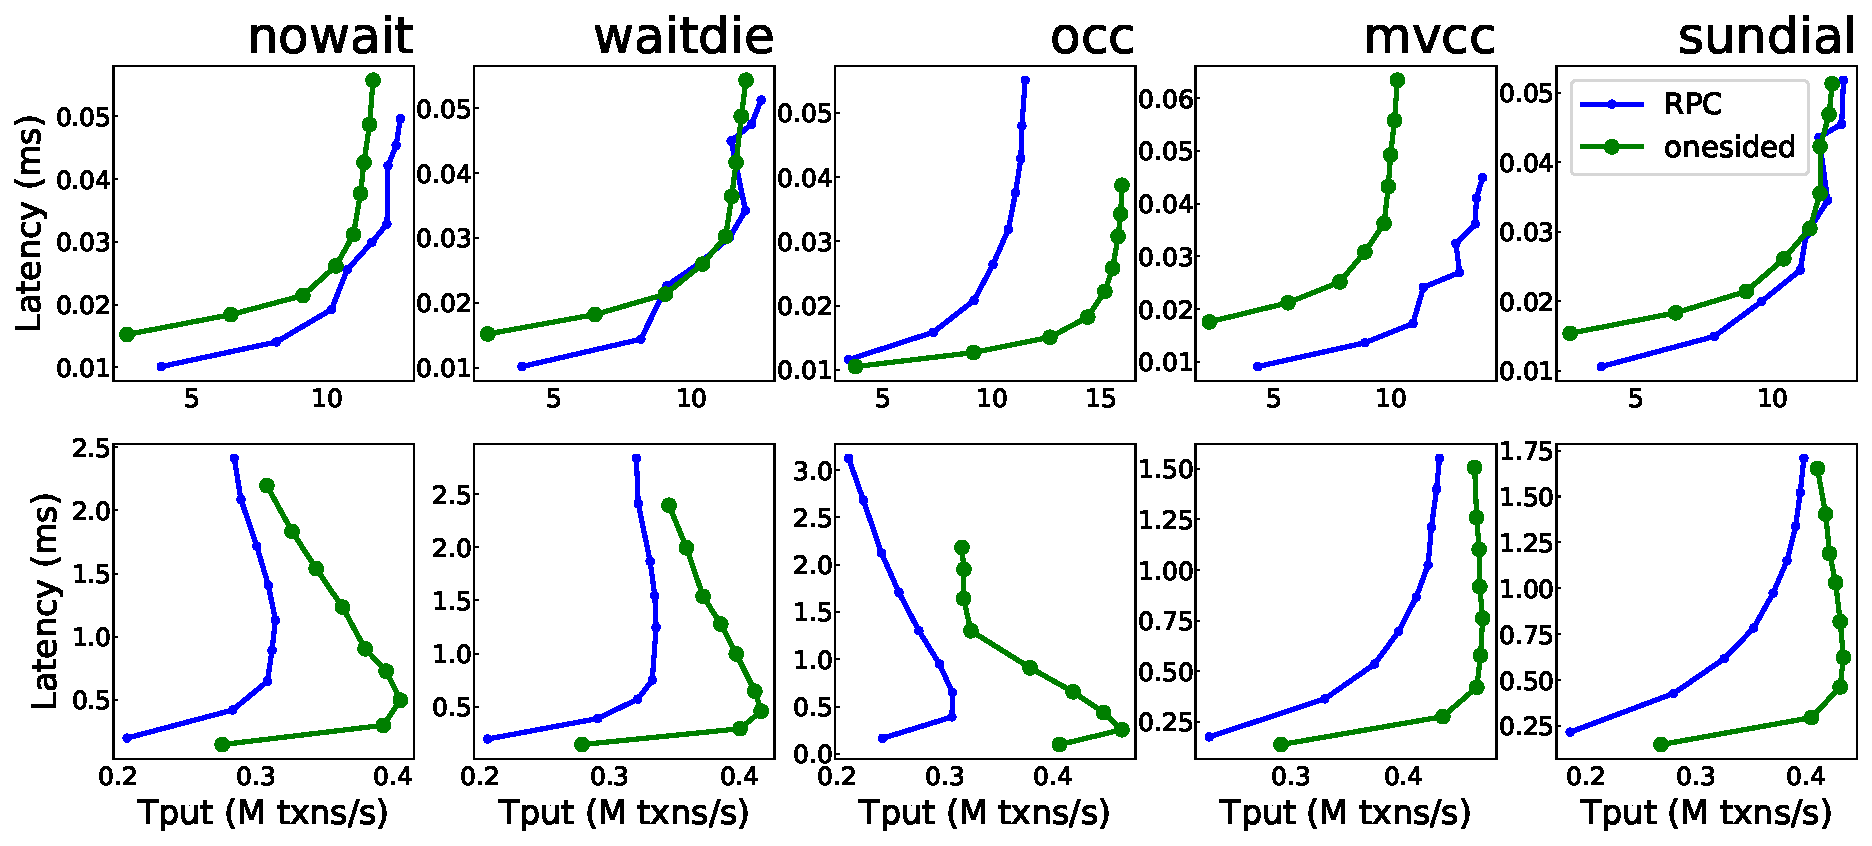
\includegraphics[width=8.5cm]{RCC-ISCA2020/images/latency-tput.pdf}
    \vspace{-0.4cm}
    \caption{Throughput and Latency for \textbf{SmallBank} (Up) and \textbf{YCSB} (Down) with co-routines ranging from 1 to 17 and a step of 2.}
    % \vspace{-0.2cm}
    \label{fig:coroutine-latency-tput}
\end{figure}

\begin{figure}[b]
    \centering
    \vspace{-0.6cm}
    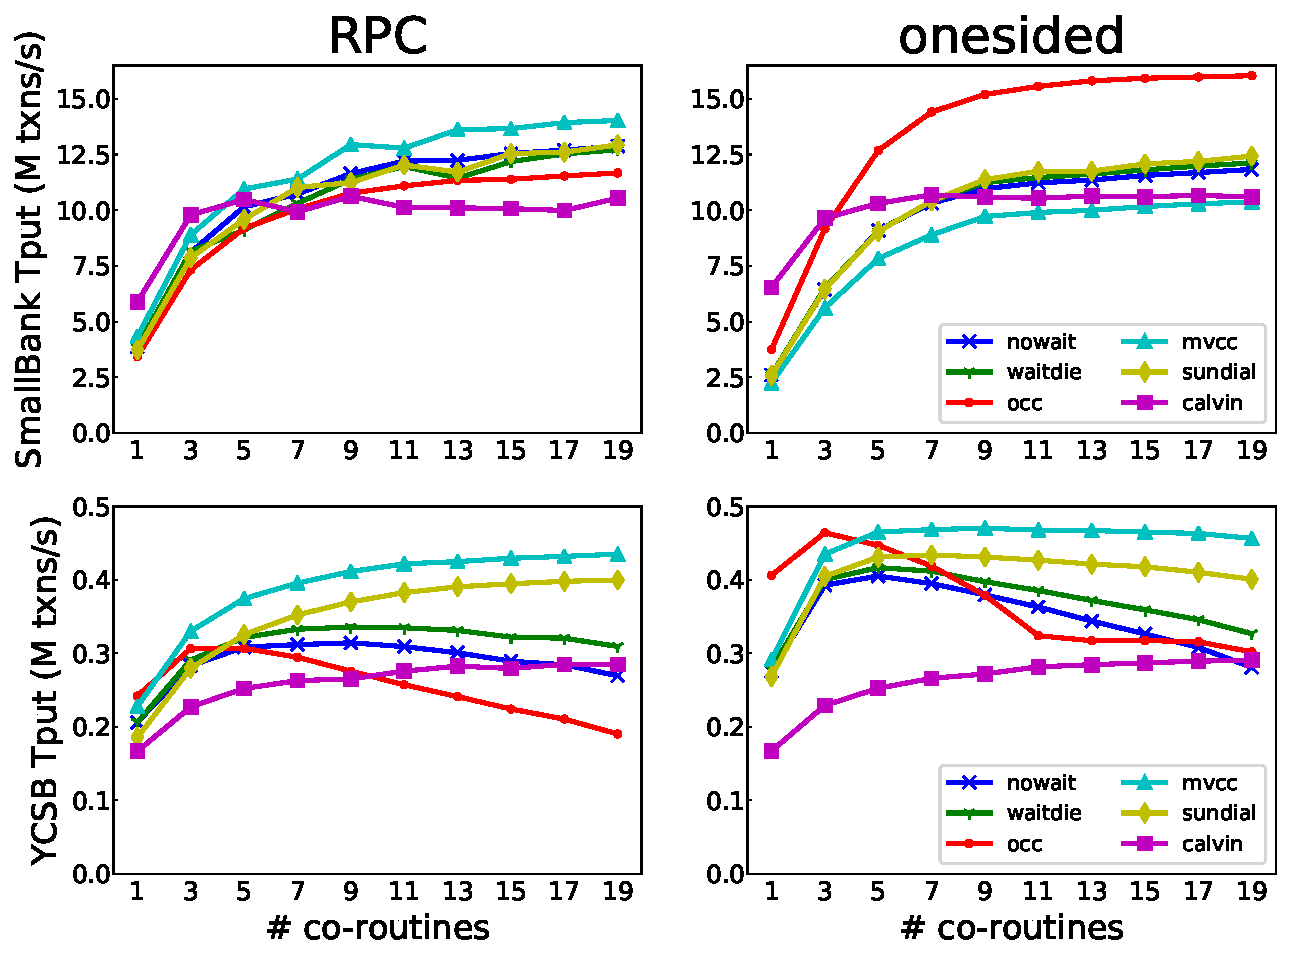
\includegraphics[width=0.8\linewidth]{images/eval_coroutines.pdf}
    \vspace{-0.4cm}
    \caption{The impact of \#co-routine to throughput}
    \vspace{-0.2cm}
    \label{fig:eval_cor_curve}
\end{figure}

To understand how co-routines affect the performance, we increase the co-routines from 1 to 17/19 with a step of 2 to test the latency and throughput in both SmallBank and YCSB. Results are reported on the EDR cluster. 

%\begin{tcolorbox}
\underline{\bf Finding 4}: The number of co-routines has great impact on the throughput and latency of both \textbf{RPC} and \textbf{one-sided} protocols while the best number of co-routines vary for different protocol implementations and different workloads. \projectname can provide a clear conclusion in making this design decision when building new transaction systems.
%\end{tcolorbox}

As seen in Figure~\ref{fig:coroutine-latency-tput}, on one hand, increasing the number of co-routines can help hide the latency of network operations, thus may improve throughput to some point. On the other hand, it will largely increase the latency of each transaction, leading to higher contention. This is because the tuples are locked for a longer time (2PL) or more likely to be interrupted for its longer life span (OCC). These two factors have different effects on SmallBank and YCSB.

As seen in Figure~\ref{fig:eval_cor_curve}, for SmallBank, the throughput of both \textbf{RPC} and \textbf{onesided} grow with the number of co-routines. As SmallBank is a network-intensive application, co-routines can greatly improve the throughput by overlapping the waiting time of network operations with transaction execution. As SmallBank touches few tuples in one transaction, there are even fewer tuples locked at the same time for \nowait and \waitdie, and the transaction has a shorter life span for \occ. Overall, the overlapping serves as the principal reason why throughput grows as \projectname uses an increasing number of co-routines. \textbf{Onesided} \occ has the most rapid growth in throughput because it locks records only at commit time, thus incurring the least conflict as co-routines increase. For \textbf{onesided} \mvcc and \sundial, which use more network operations for lower abort rate, the throughput is lower than that of the trivial protocols efficiently implemented in \textbf{onesided}.


For YCSB, which has more operations (i.e., 10) compared to SmallBank, more tuples are locked at the same time. Meanwhile, each transaction takes more time to finish, making records be locked even longer. Under this scenario, using more co-routines may significantly increase contention and adversely affect throughput after a critical point for some protocols, as seen in Figure~\ref{fig:coroutine-latency-tput} and Figure~\ref{fig:eval_cor_curve}. Among \textbf{RPC} implementations of all protocols, for those that can better handle read-write conflicts, i.e., \mvcc and \sundial, their throughput can continue growing as the number of co-routines increases. Recall that \mvcc keeps old versions for read operations and that \sundial dynamically chooses the transaction timestamp and updates the read lease. But protocols like \nowait and \waitdie, which lock all tuples involved in read and write operations, suffer from longer locked tuples with more co-routines. \occ 
is designed for the low contention scenario. 
%is aimed at performing efficiently when there is not much conflict. 
As we mentioned before, with more computation in the execution stage \occ has higher abort cost. So increasing the number of co-routines exacerbates its performance. \calvin performance is mainly bounded by the computation, because each coordinator that actively participates in a transaction has to perform the time-consuming execution stage even the transaction was not initiated by its own sequencing stage, leading to lower effective throughput. 

Comparing the execution of \nowait, \waitdie and \occ implementations on SmallBank and YCSB, we observe that the optimal co-routine number gets smaller as a transaction touches more records. \projectname can draw useful conclusions as such for future RDMA-based transaction system builders when they consider optimizing system throughput.

\vspace{-2mm}
\subsection{Impact of Contention Level}
 \vspace{-2mm}



To show how well RDMA-based protocols can handle contention, we compare the throughput of six protocols with different contention levels for YCSB. We control the contention levels by varying the possibility of one read or write visiting a small portion of data records, i.e., hot area. 
% Another parameter is the read/write ratio for one transaction. In our experiments, the read/write ratio is 1:4.
% Moreover, we also simulate execution stage by doing dummy computation which takes 5\% of the total latency of a full transaction.
The results (on EDR cluster) are shown in Figure~\ref{fig:eval_conflict_level}. 


\begin{figure}[htp]
    \centering
    \vspace{-0.2cm}
    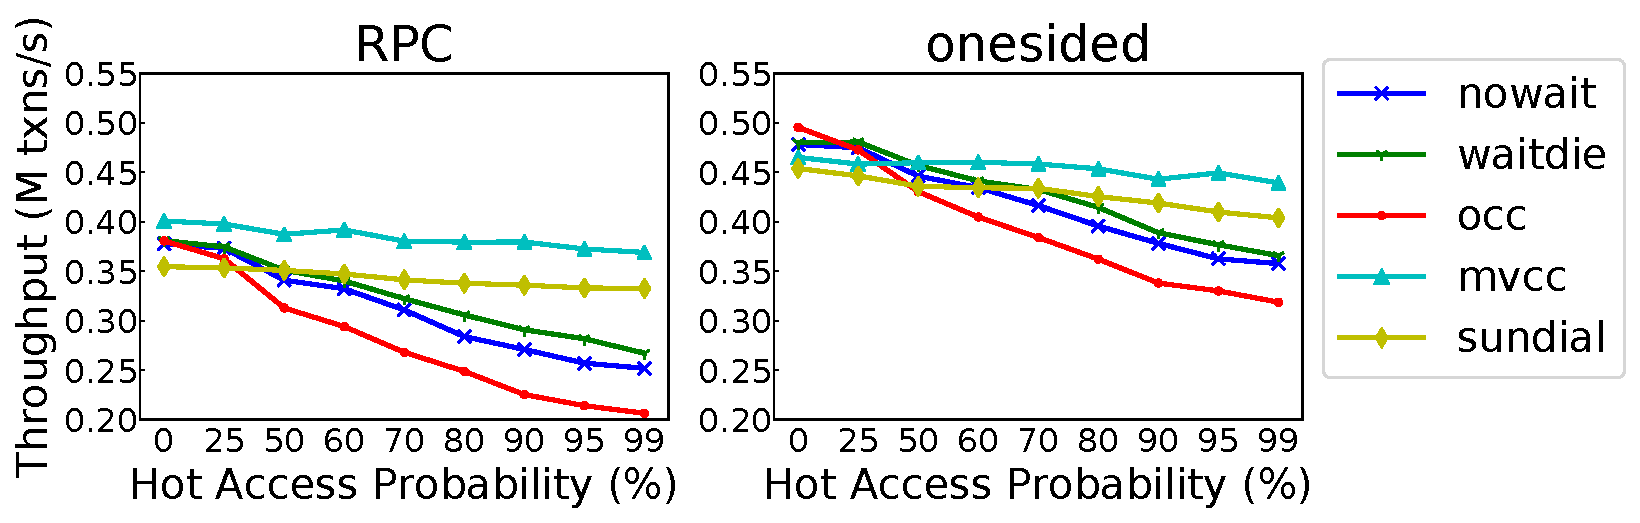
\includegraphics[width=0.8\linewidth]{images/eval_conflict.pdf}
    \vspace{-0.4cm}
    \caption{The impact of contention level to throughput for YCSB}
    \vspace{-0.8cm}
    \label{fig:eval_conflict_level}
\end{figure}

%\begin{tcolorbox}
\underline{\bf Finding 5}: The throughput of different protocol implementations drop at different rates for both \textbf{RPC} and \textbf{onesided}. \mvcc \textit{always} outperforms the state-of-the-art \sundial irrespective of contention levels.
%\end{tcolorbox}

In both \textbf{RPC} and \textbf{onesided} implementations, performance of \occ decreases most sharply because of larger possibility to abort and high abort cost due to its optimistic assumption under a high contention level. The performance of \nowait and \waitdie significantly decrease due to the intensive conflict read and write locks. \mvcc and \sundial are less affected when the conflict rate increases; their throughput decrease is slow because they have optimization to avoid read-write conflict. \calvin is not affected much by different contention levels because a \calvin transaction only locks local records for a short period without necessarily waiting for remote locks. This behavior of \calvin is confirmed in~\cite{Thomson:2012:CFD:2213836.2213838}.

%The effect brought by conflict rate similarly effect the \textbf{onesided} and \textbf{rpc} version, because the performance difference mainly come from the algorithm here.
We also notice that \textbf{onesided} \sundial and \mvcc, although featuring good read-write conflict management, are worse than \textbf{onesided} \occ when a transaction has the least conflict rate. That is because these two have more complicated operations to maintain more information to reduce the abort rate, which is more costly because every access to remote data will trigger network operation in \textbf{onesided} version.

%\blue{TODO: \calvin and contention}

It is worthwhile to note that \mvcc is consistently better than \sundial irrespective of contention levels in both \textbf{RPC} and \textbf{onesided} implementations for YCSB. While we do not expect \cite{yu2018sundial} to compare with all previous concurrency control protocols under all possible workloads, our \projectname's results show a strong indication that \sundial is worse than one variant of \mvcc implementations when the workload is computation-intensive in the RDMA context. This non-trivial observation would not possible without our unified RDMA-based concurrency control framework. 

\vspace{-2mm}
\subsection{Impact of Execution Workloads}
%\vspace{-2mm}

\begin{figure}[htp]
    \centering
    \vspace{-0.2cm}
    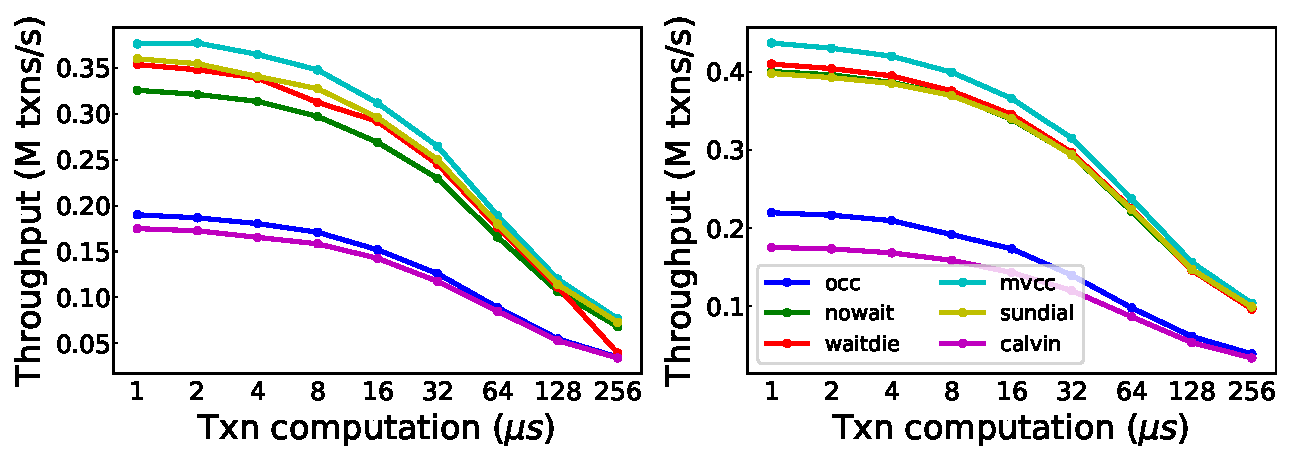
\includegraphics[width=0.8\linewidth]{images/eval_exe_workload.pdf}
    \vspace{-0.4cm}
    \caption{The impact of computation workload to throughput}
    \vspace{-0.2cm}
    \label{fig:eval_sleep_curve}
\end{figure}

% As shown in the overall results, \textbf{onesided} version can better handle transactions bounded by computation. 
%So we increase the percentage of the computation in one transaction. 
To study the implication of computation ratio, we add dummy computation in the execution stage of YCSB, ranging from 1 to 256 $\mu$s. We carry out experiments on the EDR cluster and show results in Figure~\ref{fig:eval_sleep_curve}.

%\begin{tcolorbox}
\underline{\bf Finding 6}: \textbf{RPC} and \textbf{onesided} share similar decreasing trend with increasing computation workload at execution stage; \textbf{onesided} always outperforms \textbf{RPC} for different computation workloads.
%\end{tcolorbox}

%We can see the same trend that the throughput decrease with increasing computation at execution stage for . Yet \textbf{onesided} version always outperforms \textbf{rpc} version under different computation workloads. 

%Moreover, \textbf{onesided} version have a slower decreasing trend. 

In \textbf{RPC} versions, more computation time on the execution stage causes higher latency for an RPC request to get handled, which significantly increases the time that a tuple is locked, leading to higher abort rate. \textbf{onesided} versions are also adversely affected yet have a relatively slower decreasing trend. 
Suffering from both high abort cost and long computation time, \occ performs much worse than 2PL protocols. \calvin's performance is bounded by local computation; thus, there is no difference between {\bf RPC} and \textbf{onesided} version.






% -- For the following sections, please check OSDI and VLDB papers carefully and try to include all results we can get similar to them. We can organize sections later. 

% -- We can first include all experiments summarized by Kezhao, and go over again **each** result figure of the two papers, and ask whether we can get it and whether it is needed (or how can several be combined into one)? We want to provide a superset of results
% compared to the two. We should pay special attention to the findings **unknown** before or **unexpected**.

% -- We will not have a "discussion" section after the Evaluation, instead you need to analyze the results in detail in each subsection here. 

% \begin{figure}[htp]
%     \centering
%     \includegraphics[width=6cm]{images/overall_throughput_10thread_10_cor.pdf}
%     \caption{Overall Throughput}
%     \label{fig:overall_tput}
% \end{figure}

% \begin{figure}[htp]
%     \centering
%     \includegraphics[width=6cm]{images/overall_abort_10thread_10_cor.pdf}
%     \caption{Overall Abort Rate}
%     \label{fig:overall_abort}
% \end{figure}


% \begin{figure}
%   \centering
%   \begin{tabular}{@{}c@{}}
%     \includegraphics[width=.8\linewidth,height=50pt]{images/latency_of_operations_small_bank_10_thread_1_cor.pdf} \\[\abovecaptionskip]
%     \small (a) 10 threads 1 co-routine
%   \end{tabular}

%   \vspace{\floatsep}

%   \begin{tabular}{@{}c@{}}
%     \includegraphics[width=.8\linewidth,height=50pt]{images/latency_of_operations_small_bank_10_thread_5_cor.pdf} \\[\abovecaptionskip]
%     \small (b) 10 threads 5 co-routines
%   \end{tabular}
  
%   \begin{tabular}{@{}c@{}}
%     \includegraphics[width=.8\linewidth,height=50pt]{images/latency_of_operations_small_bank_10_thread_10_cor.pdf} \\[\abovecaptionskip]
%     \small (b) 10 threads 10 co-routines
%   \end{tabular}
  
%   \begin{tabular}{@{}c@{}}
%     \includegraphics[width=.8\linewidth,height=50pt]{images/latency_of_operations_small_bank_10_thread_15_cor.pdf} \\[\abovecaptionskip]
%     \small (b) 10 threads 15 co-routines
%   \end{tabular}

%   \caption{Latency break down in small bank}\label{fig:lat_break_down}
% \end{figure}

% \begin{figure}
%   \centering
%   \begin{tabular}{@{}c@{}}
%     \includegraphics[width=.8\linewidth,height=50pt]{images/latencyycsb_cor1.pdf} \\[\abovecaptionskip]
%     \small (a) 10 threads 1 co-routine
%   \end{tabular}

%   \vspace{\floatsep}

%   \begin{tabular}{@{}c@{}}
%     \includegraphics[width=.8\linewidth,height=50pt]{images/latencyycsb_cor5.pdf} \\[\abovecaptionskip]
%     \small (b) 10 threads 5 co-routines
%   \end{tabular}
  
%   \begin{tabular}{@{}c@{}}
%     \includegraphics[width=.8\linewidth,height=50pt]{images/latencyycsb_cor10.pdf} \\[\abovecaptionskip]
%     \small (b) 10 threads 10 co-routines
%   \end{tabular}
  
%   \begin{tabular}{@{}c@{}}
%     \includegraphics[width=.8\linewidth,height=50pt]{images/latencyycsb_cor15.pdf} \\[\abovecaptionskip]
%     \small (b) 10 threads 15 co-routines
%   \end{tabular}

%   \caption{Latency break down in YCSB}\label{fig:lat_break_down}
% \end{figure}


% \begin{figure}
%   \centering
%   \begin{tabular}{@{}c@{}}
%     \includegraphics[width=.9\linewidth,height=50pt]{images/latency_of_operations_small_bank_10_thread_1_cor.pdf} \\[\abovecaptionskip]
%     \small (a) 10 threads 1 co-routine smallbank
%   \end{tabular}

%   \vspace{\floatsep}

%   \begin{tabular}{@{}c@{}}
%     \includegraphics[width=.9\linewidth,height=50pt]{images/latencyycsb_cor1.pdf} \\[\abovecaptionskip]
%     \small (b) 10 threads 1 co-routines YCSB
%   \end{tabular}
%   \caption{Latency break down}\label{fig:lat_break_down}
% \end{figure}

% We tested the break down time cost in each stage of five protocols with co-routine number ranging from 1 to 15 in small bank and YCSB. We can see that RPC and \textbf{onesided} version have very different performance between small bank and YCSB. In small bank, with different co-routine number, RPC always outperforms \textbf{onesided} in read and lock\&read. This is because in out RPC implementation, a read can be done by launching just one RPC request. No matter if the stage needs complex operations(for example in MVCC, it should traverse all the time stamps and find the suitable one to read), RPC handler can locally access the data and check the time stamps. However, for \textbf{onesided}, any data access will be remote so as to be costly. Especially when \textbf{onesided} has to check the correctness of data, it should re-read the write time stamp after reading the real data, to guarantee the atomicity of reading. In this case, two RDMA read requests will be launched. For lock\&read operation, for protocols using waitdie deadlock prevention method, once a lock fails and the one with high priority would retry. For \textbf{onesided}, one retry means one RDMA atomic operation. But for RPC, the retry can be done locally within the handler. High contention will lead to more RDMA atomic requests for retry, causing heavier network traffic. The side effect also show on the throughput results. As a result in small bank and TPCC, the RPC of different protocols all outperform \textbf{onesided} with similar abort rate. 

% However, in YCSB with execution phase, we have the different results. Latency of RPC is at least three times higher than \textbf{onesided} version. We add some dummy execution workload into YCSB which takes 25\% of the whole transaction time to simulate excution in real-world transaction. And in this time, the CPU will be busy and become the bottleneck of the process. In the RPC version, the RPC requests should be handled by the remote node. As the remote node is busy doing the tasks in the execution phase, in average it will take much longer time for the handler to handle the RPC request. But for \textbf{onesided} version, as the one-sided operations bypass the remote CPU, the latency remains the same with the transactions in the benchmarks that are with low CPU utilization. In this condition, \textbf{onesided} outperforms RPC in both latency and throughput.

\vspace{-2mm}
\subsection{System Resource Utilization}
%\vspace{-2mm}

%\begin{tcolorbox}
\underline{\bf Finding 7}: \textbf{Onesided} implementations are less likely to be bottlenecked by system resources and can reach much higher network utilization than their \textbf{RPC} counterparts.
%\end{tcolorbox}

We measure system resource utilization of both \textbf{RPC} and \textbf{onesided} implementations by two experiments. First, we use two different thread numbers (i.e., five threads and ten threads) of all implementations on the EDR cluster for the YCSB benchmark and show the throughput increase in Table~\ref{tbl:two-threads}. Since our \projectname is symmetric: i.e., each co-routine in some thread only communicates with another co-routine at the {\em same thread} of another machine. Ideally, doubling thread numbers would also doubling the throughput increase if not bottlenecked by system resources and if we did not consider the effect of an increased contention level. In reality, from Table~\ref{tbl:two-threads}, we can see that \textbf{onesided} implementations are equally or more closer to the ideal case, thus having equal or less likelihood of being bottlenecked by system resources as \textbf{RPC} implementations. This behavior is understandable since \textbf{onesided} implementations bypass system calls and kernels, thus avoiding many possibilities of being bottlenecked. \textbf{Onesided} \sundial is the protocol that is closest to linear scalability in \projectname. Overall, \projectname provides researchers with the opportunity to compare RDMA-based protocols in terms of system utilization. We leave pinpointing the exact system resource bottleneck for each protocol as an important future work.

Second, to characterize the network utilization of different protocols in both \textbf{RPC} and \textbf{onesided} implementations, we measure their message rates in \projectname when executing for the YCSB workload on the EDR cluster. Table~\ref{tbl:message-rate} shows our results. We observe the max message rate in RCC reaches 31.06 Mpps by \textbf{onesided} \nowait. Given that the RDMA peak message rate of our {EDR} cluster is 33 Mpps, \textbf{onesided} \nowait has reached 94.1\% of the peak. On average \textbf{onesided} implementations send approximate {\em twice} more packages per second than their \textbf{RPC} counterparts, which indicates that \textbf{onesided} protocols all have much higher network utilization. 




% We believe in a cluster with lower network performance, RCC can show different bottlenecks.



\subsection{Stage Latency Breakdown}

While we have already done some experiments to compare various aspects of different protocols in \projectname. Previous latency results are still not an accurate reflection of the actual bottleneck of each protocol since interleaving transactions among multiple co-routines increases transaction latency nondeterministically. In order to pinpoint the stage-wise bottleneck of each protocol implementation further, we run all implementations except \calvin using {\em only one} co-routine for SmallBank on 4 nodes of {EDR} cluster and break down a whole transaction latency into different stages: \textit{Read}, \textit{Lock}, \textit{Release}, \textit{Commit}. \sundial has an extra lease \textit{Renew} latency. \calvin is not included in this experiment because all these stages are local operations for \calvin. Figure~\ref{fig:latency-breakdown} shows the stage-wise latency breakdown. Note that for \textbf{RPC} \nowait and \waitdie, a record is returned together with locking result (as a  whole tuple), so their \textit{Read} latency is combined into the \textit{Lock} latency.

\begin{table}[h!]
\vspace{-2mm}
\caption{Thoughput in K/s for different threads on EDR}
\vspace{-2mm}
\centering
\begin{tabular}{|c|c|c|c|c|c|c|}
 \hline
  &
 \multicolumn{3}{|c|}{\textbf{RPC}} &
 \multicolumn{3}{|c|}{\textbf{onesided}} \\
 \hline
 \#threads & 5 & 10 & & 5 & 10 & \\
 \hline
 nowait & 40.23	& 67.9 & 1.69x &	56.83 & 107.44 & 1.89x \\
 \hline
 waitdie & 40.12 & 71.69 & 1.79x & 57.26 & 102.08 & 1.78x \\
 \hline
 occ & 27.45 & 48.09 & 1.75x & 47.93 & 84.53 & 1.76x \\
 \hline
 mvcc & 52.34 & 91.93 & 1.76x & 68.16 & 125.61 & 1.84x \\
 \hline
 sundial & 50.28 & 80.68 & 1.60x & 60.26 & 119.19 & 1.98x \\
 \hline
\end{tabular}
\label{tbl:two-threads}
\end{table}


\begin{table}[h!]
\vspace{-0mm}
\caption{Msg. Rate in M pkgs/s on EDR and utilization}
\vspace{-3mm}
\centering
\begin{tabular}{|c|c|c|c|}
 \hline
  &
 \textbf{RPC} & 
 \textbf{onesided} & network utilization \% \\
 \hline
 nowait & 9.49 & 31.06 & $28.8 \rightarrow 94.1$ \\
 \hline
 waitdie & 9.25	& 30.77 &  $28.0 \rightarrow 93.2$ \\
 \hline
 occ & 9.75 & 30.38 & $29.5 \rightarrow 92.1$   \\
 \hline
 mvcc & 10.70 & 28.46 & $32.4 \rightarrow 86.2$ \\
 \hline
 sundial & 9.91	& 29.52 & $30.0 \rightarrow 89.5$  \\
 \hline
\end{tabular}
\vspace{-0mm}
\label{tbl:message-rate}
\end{table}

For \textbf{RPC} implementations, as illustrated in Figure~\ref{fig:latency-breakdown}, \mvcc incurs the largest \textit{Read} latency due to the participant's traversal of the all \texttt{wts} of the requested record. \mvcc also incurs the largest \textit{Lock} latency due to the participant's double checking of conditions for successful locking. \occ incurs the largest latency at \textit{Commit} and \textit{Release} stages and second largest \textit{Read} latency compared to other protocols. This is because the \occ implementation of \cite{wei2018deconstructing} accumulates all RPC read/write messages in one stage into one message before broadcasting it to all participants, which uses higher network bandwidth and incurs larger latency (This latency is not apparent with ten co-routines as in Figure~\ref{fig:eval_overall}). 

For \textbf{onesided} implementations, as illustrated in Figure~\ref{fig:latency-breakdown}, \textit{Release} is not the bottleneck for any protocol. \mvcc and \sundial suffers from the top-2 \textit{Read} latency due to their extra logic for ensuring valid record version or valid lease upon read operations. \mvcc suffers from the largest \textit{Lock} latency since it needs to retrieve longer metadata upon locking using \texttt{CAS}. 
%\occ suffers from the largest \textit{Release} and \textit{Commit} latency since \red{xxx}.

By analyzing stage latency results, researchers can make use of \projectname to understand better and mitigate the stage-wise bottlenecks of \textbf{RPC} and \textbf{onesided} implementations.

\vspace{-2mm}
\subsection{Comparison with the State-of-the-art}
\vspace{-2mm}

As we have stated that \projectname is the {\em first} unified framework of RDMA-based implementations of representative protocols. There is no apple-to-apple comparison for each protocol. We implemented five TCP-based RPC versions in \projectname and compared these TCP protocols in \projectname with corresponding TCP-based protocols in \cite{harding2017evaluation} and \cite{yu2018sundial}  using similar configurations on YCSB. Table~\ref{tbl:compare-with-stoa} shows the results.
As we can see, except \sundial, our TCP implementations are comparable or better than corresponding implementations in \cite{harding2017evaluation}. The two-sided RDMA versions in \projectname perform an order of magnitude better than corresponding TCP versions in \projectname or \cite{harding2017evaluation}.



\begin{table}[h!]
\vspace{-2mm}
\caption{Comparing throughput (Txns/s) of \projectname with the State-of-the-Art protocol implementations using TCP. }
\vspace{-2mm}
\centering
\begin{tabular}{|c|c|c|c|}
 \hline
  &
 Other TCP-based 
  & 
 \projectname TCP-based
  &
 \projectname Two-sided  
 \\
 \hline
 nowait & approx. 50000~\cite{harding2017evaluation} & 48394 & 308177 \\
 \hline
 waitdie & approx. 10000~\cite{harding2017evaluation} & 51444 & 336514 \\
 \hline
 occ & approx. 40000~\cite{harding2017evaluation} & 49949 & 257307 \\
 \hline
 mvcc & approx. 20000~\cite{harding2017evaluation} & 63514 & 420000 \\
 \hline
 sundial & approx. 70000~\cite{yu2018sundial} & 38275 & 383237 \\
 \hline
 % calvin & ~120000~\cite{harding2017evaluation} & - & 281426 \\
%  \hline
\end{tabular}
\vspace{-0.4cm}
\label{tbl:compare-with-stoa}
\end{table}

\begin{figure}[h]
    \centering
    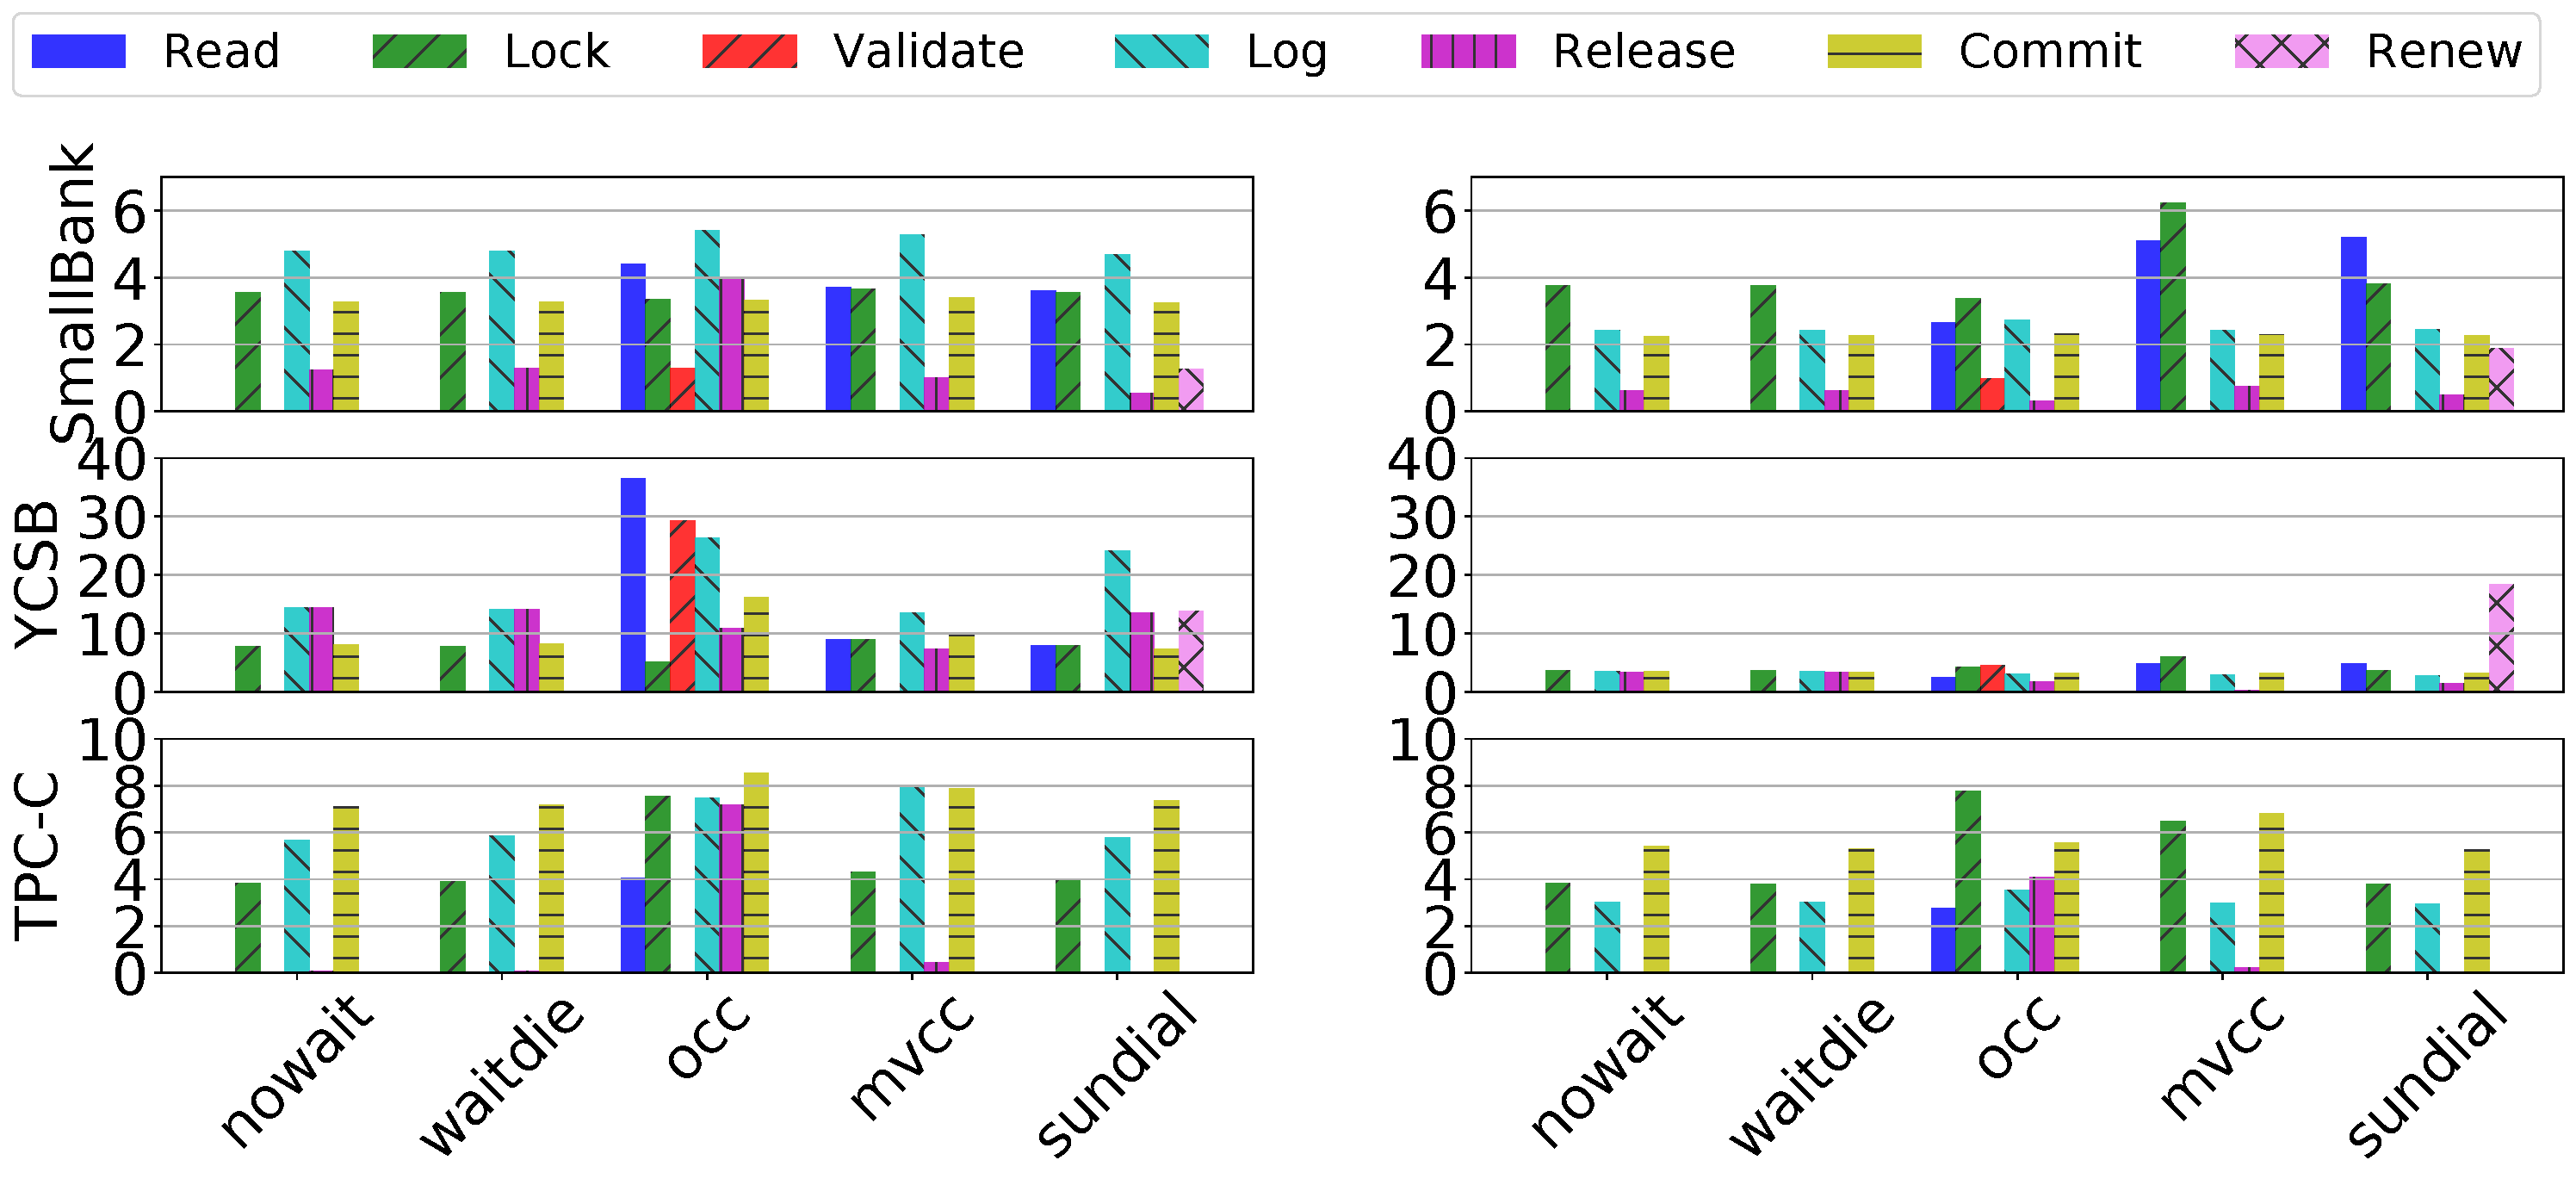
\includegraphics[width=0.8\linewidth]{RCC-ISCA2020/images/lat_breakdown.pdf}
    \vspace{-0.4cm}
    \caption{Latency breakdown for \textbf{RPC} (Left) and \textbf{onesided} (Right)}
    \vspace{-0.6cm}
    \label{fig:latency-breakdown}
\end{figure}
